
\chapter{Datasets}
\section{Datasets used in LFV analysis}
\subsection{\Hmuhad}
The data sample used in the analysis is from LHC 2016 Runs, recorded by CMS detecter. Total integrated luminosity of the analyzed data is $35.9 ~\textrm{fb}^{-1} $ with center-of-mass energy of $ \sqrt{s}=13 ~\textrm{TeV} $. The data sample labeled in the CMS experiment as SingleMuon\_Run2016B,C,D,E,F,G,H. The name SingleMuon in the data sample represents the trigger used in the analysis, which selects the events with at least a muon passed the trigger selection. Gluon gluon fusion Higgs(ggH)~\cite{Georgi:1977gs} production and vector boson fusion Higgs(VBF)~\cite{Cahn:1986zv} are the main Higgs production channels considered in the analysis. For the background samples, besides the misidentified background which is talked about in detail in Chapter6, the other background samples are all generated with Monte Carlo(MC) simulation.  POWHEG~\cite{POWHEG-BOX} or MadGraph~\cite{Alwall:2014} generator is used for the generation and all of the MC samples, including the signal samples, the parton showering, fragmentation, and decays are performed by Pythia8~\cite{Sjostrand:2014zea}.  Pileup effect is taking into account in the generator by generate minimum bias events simultaneously and a correction is applied by comparing the data sample. The average number of pileup interaction per bunch crossing is 27. CMS detector environment is simulated by GEANT4~\cite{GEANT4}. The details of the MC samples used in the analysis are summarized in Table.~\ref{tab:mutaumcsamples} and Table.~\ref{tab:mutaumcsamples2}.

\begin{table}[!hbpt]
\caption{Monte Carlo samples used in the search, together with their respective cross sections.}
\begin{center}
% sample name   &    generator    & cross section 
\begin{tabular}{|c|c|c|}
\hline
Processes & Generator & Cross section [pb] \\\hline
DYJets$\to\ell \ell$, $m_{\ell \ell}>50$ GeV &MadGraph+pythia8   & 4954.0 \\\hline
DY1Jets$\to\ell \ell$, $m_{\ell \ell}>50$ GeV &MadGraph+pythia8 & 1012.5 \\\hline
DY2Jets$\to\ell \ell$, $m_{\ell \ell}>50$ GeV&MadGraph+pythia8  & 332.8 \\\hline
DY3Jets$\to\ell \ell$, $m_{\ell \ell}>50$ GeV&MadGraph+pythia8  & 101.8 \\\hline
DY4Jets$\to\ell \ell$, $m_{\ell \ell}>50$ GeV&MadGraph+pythia8  & 54.8 \\\hline
DYJets$\to\ell \ell$, $m_{\ell \ell}<50$ GeV&MadGraph+pythia8    & 1861.0 \\\hline
$t\bar{t}$                                                     & powheg+PYTHIA     &  831.76\\\hline
$t \backslash \bar{t}\to t w$                        & powheg+PYTHIA8     &  35.85 \\\hline
$WZ \to \ell 3v$                                          & MadGraph+PYTHIA8   &  3.05   \\\hline
$WZ \to \ell v 2q $                                      & MadGraph+PYTHIA8   &  10.71  \\\hline
$WZ \to 2 \ell 2q $                                      &  MadGraph+PYTHIA8  &  5.595 \\\hline
$t\to4f $                                                     & POWHEG+PYTHIA8       & 136.02\\\hline
$\bar{t}\to4f $                                             & POWHEG+PYTHIA8       & 80.95\\\hline
$WW \to \ell v 2q$                                      & MadGraph+PYTHIA8   &  1.212   \\\hline
$ZZ \to 2\ell 2q $                                        & MadGraph+PYTHIA8    &  3.22   \\\hline
$VV \to2\ell 2 q$                                        &  MadGraph+PYTHIA8   &  11.95  \\\hline

\end{tabular}
\end{center}
\label{tab:mutaumcsamples}
\end{table}

\begin{table}[!hbpt]
\caption{Continue with MC samples used in the analysis.}
\begin{center}
\begin{tabular}{|c|c|c|}
\hline
MC simulations & Generator & Cross section [pb] \\\hline
$VV \to2\ell 2 q$                                        &  MadGraph+PYTHIA8   &  11.95  \\\hline
$ggH\to \Pgt\Pgt $                                      & POWHEG+PYTHIA8 &      3.046\\\hline
$\textrm{VBF}H\to \Pgt\Pgt $                     & POWHEG+PYTHIA8 &      0.237\\\hline
$ggH\to WW \to 2\ell 2v$                            & POWHEG+PYTHIA8 &      1.103\\\hline
$\textrm{VBF}H\to WW\to 2\Pl 2v$             & POWHEG+PYTHIA8 &    0.086\\\hline
$ZH \to \Pgt\Pgt$                                        & POWHEG+PYTHIA8 &    0.055\\\hline  
$W^{-}\backslash W^{+} H\to\Pgt\Pgt$        & POWHEG+PYTHIA8 &    0.086\\\hline 
$ttHJet \to \Pgt\Pgt$                                   &MadGraph+PYTHIA8&     0.32\\\hline   
\end{tabular}
\end{center}
\label{tab:mutaumcsamples2}
\end{table}


\subsection{\Hehad}

The search of lepton flavour violation Higgs decay $\Hehad$  is performed with CMS 2012 RunI dataset at center-of-mass energy  $\sqrt{s}=8 ~\textrm{TeV}$. The dataset is named as SingleElectron\_Run2012A,B,C,D with an integrated luminosity of $19.7 ~\textrm{fb}^{-1}$. Single electron HLT tigger is used which is talked more in details in Chapter 5. A detail list of simulation samples used in the analysis is listed in Table.~\ref{tab:mcdatasets}.  For the signal samples, ggH and VBF Higgs production channels are the main channels considered. For background samples, besides $Z\to \tau \tau$ which is produced with embedding technique and misidentified background which is estimated with data-driven method are produced with MC simulation. Various simulation packages are used. Signal samples are produced with PYTHIA8, which uses sophisticated $\tau$-lepton decay machinery. Tauola~\cite{Simulation:Tauola} is also used for the simulation of $\tau$ lepton decay in some of samples. CMS detector environment is simulated by GEANT4. 


\begin{table}[hbtp]
 \begin{center}
  \caption{Signal and background MC samples}
  \label{tab:mcdatasets}
  \begin{tabular}{l|l|l}
Processes & Generator & Cross section [pb] \\\hline
$ggH\to e\tau $     &          PYTHIA8                     &  19.27                \\\hline
$VBH\to e\tau$     &          PYTHIA8                      &   1.58                \\  \hline
$ggH \to \tau\tau$ &POWHEG+PYTHIA6              &  19.27           \\\hline
 $VBF\to\tau\tau$  &POWHEG+PYTHIA6              &   1.58           \\  \hline
$t\overline{t}+\textrm{jets}~ \textrm{full}~\textrm{leptonic}$  &  MadGraph+Tauola                &  26.20                \\\hline
$t\overline{t}+\textrm{jets}~\textrm{Semi}~\textrm{leptonic}$   & MadGraph+Tauola           &  109.28               \\ \hline
$t \to tw$              &   POWHEG+Tauola     &    56.4 \\\hline
$\bar{t} \to tw$              &   POWHEG+Tauola     &    30.7 \\\hline
$t$,$\bar{t}(\textrm{T channel})$           & POWHEG+Tauola        &   11.1 (11.1)          \\ \hline
$WW \to 2l2\nu+jets$    & PYTHIA6+Tauola                  & 5.824\\ \hline
$ZZ\to 4l$               & MadGraph+Tauola                 & 0.18                  \\  \hline
$ZZ\to 2l2Q$             &MadGraph+Tauola              &   2.502               \\  \hline
$ZZ\to 2l2\nu$           &MadGraph+Tauola              &    0.716              \\  \hline
$WZ\to 2l2Q$             &MadGraph+Tauola                &    2.21               \\  \hline
$WZ\to 3l\nu$            &MadGraph+Tauola           & 1.06                  \\  \hline
  \end{tabular}
 \end{center}
\end{table}





\section{Event reconstruction}
In this section, a general presentation of the event reconstruction algorithm used in CMS, particle-flow(PF) reconstruction is shown. A more detail information about the reconstruction of tracks and the objects related to the lepton flavour violation higgs decay are in the following section. 
\subsection{Particle flow algorithm}

Particle flow event reconstruction algorithm is the main algorithm used in CMS. PF performs a global event reconstruction~\cite{CMS-PRF-14-001}, which aim to utilize the information from the whole detector to identify individual particles in each event.



\subsubsection{Tracking and Calorimeter algorithm}\label{PFtracker}

In the PF algorithm, the reconstruction of charged particles in the inner tracker is a crucial part. In this section, the reconstruction of the trajectories of charged particles, especially the electron and muon reconstruction is discussed. 

Inner tracker is aimed at measuring the track of energetic charged particle. The track finder is based on the Kalman Filtering(KF)~\cite{tracker:algo}. This reconstruction comes in a couple steps. First an initial seed is generated from a couple hits that compatible with a track in the tracker, then a trajectory is builded with the seed and other hits from the tracker along this track. At last a fit is perform on the track  to determine the properties of this particle candidate, like the momentum, the charge and the direction. The qualities that can affect the performance of the reconstruction are like the number of hits in the pixel detector, the total number of hits in the tracker, the distance from the cylinder and the energy of this charged particle. This is discussed in more details later.

The performance of the track reconstruction is measured in reconstruction efficiency and misreconstruction rate. The reconstruction efficiency is defined as the ratio of track reconstructed with more than 50\% hits from simulated hits and the total simulated tracks. The misreconstruction rate is defined as the fraction of the tracks can not be associated with simulated tracks of the whole simulated tracks.  If a charged hadron is not identified by the tracking algorithm, then the hadron is take as a neutral hadron and measured by the calorimeters. This will affect the jet energy and position resolution. Improving the track reconstruction efficiency while keeping the misreconstructed rate low is critical for PF reconstruction.

In CMS, an iterative tracking is perform, in which the reconstruction of tracks is done is a couple steps. Each step is aimed for a moderate efficiency but with a high purity. After one step, the hits that used to form tracks are masked and a next step is perform. This iterative tracking is down in ten steps if necessary and the detail information is shown in Table.~\ref{tbl:iterative_tracking} and more can be found in \cite{CMS-PRF-14-001}. In the table, the name column points out the processes that that step of iteration is aiming at. The seeding column shows the requirement on the seeding, while the targeted tracks column shows the characters of the tracks.

Electron is one of the main particle understudy in $\Hehad$ search. In CMS, electron track reconstruction is taken as a merge of ECAL based and tracker based strategy. The tracker based seeding strategy is as described above, besides the case when energetic photons are radiated, then a preselection based on the number of hits and $\chi^{2}$ of the fit is set with the Gaussian-sum filter~\cite{Algo:GSF}. The ECAL based electron seeding strategy building the superclusters(SC) to gathering the bremsstrahlung photons. The energy of the SC is taken as the energy sum of the cell crystals inside and the position is evaluated with energy weight. The electron trajectory in the first layer of the the tracker is estimated and the seed from the track is selected. This works in the case when there is not much bremsstrahlung photons, then most of the energy is deposited in ECAL. In the case when soft photons are radiated mostly, ECAL based seeding may still performs well. But when the electrons are in the jets or low energy, either electron contributions are overlapping with other particle or the radiation and bending is too much, it is hard to recover these electrons with ECAL based algorithm only. The ECAL based and tracker based electron seeding is merged into one collection, which significantly improves the reconstruction efficiency.



\begin{table}[!tpb]
\caption{Iterative tracking steps take in CMS \label{tbl:iterative_tracking}}
\label{tab:antil}
\begin{center}
\begin{tabular}{|llll|}   
\hline
Iteration                   &  Name               &   Seeding            &  Targeted Tracks  \\\hline
1                              & InitialStep          & pixel triplets        &  prompt, high $p_{t}$   \\
2                              & DetachedTriplet          & pixel triplets        &  from b hadron decays, R$\lesssim$ 5 cm  \\
3                              & LowPtTriplet          & pixel triplets        &  prompt, low $p_{t}$ \\
4                              & PixelPair          & pixel pairs                &  recover high $p_{t}$ \\
5                              & MixedTriplet          & pixel+strip triplets                &  displaced,  R$\lesssim$ 7 cm   \\
6                              & PixelLess          & strip triplets / pairs               &  very displaced, R$\lesssim$ 25 cm     \\
7                              & TobTec          & strip triplets / pairs               &  very displaced, R$\lesssim$ 60 cm     \\
8                              & JetCoreRegional          & pixel+strip pairs               &  inside high $p_{t}$ jets    \\
9                              & MuonSeededInOut          & muon-tagged tracks               &  muons   \\
10                            & MuonSeededOutIn          & muon detectors                &  muons   \\\hline
\end{tabular}
\end{center}
\end{table}


Calorimeters are crucial components for the PF algorithm in CMS. The clustering algorithm in calorimeters is used to identify neutral stable particles like phone and neutral hadron, together with tracker in the identification of charged particles, reconstructing the energy of electrons and the possible associated bremsstrahlung photons and measuring the energy of charge particles that are missed by the tracker.  

The clustering algorithm is perform separately in each sub-detector system beside the HF in which each cell directly raise a cluster. The algorithm starts by finding a cluster seed. Then a topological walking around the neighbouring cells is performed. Both seed cells and neighbouring cells are required to pass certain thresholds to construct high quality candidates and suppress the contribution from noise. In ECAL endcaps, additional requirements on $E_{T}$ because of the high noise level. In each of the topological clusters, the energy for the neighbouring cells are assumed from the seed cells. A Gaussian-mixture model is used in the construction of the topological clusters to evaluate the contribution of each cells. The finally parameters of the model is obtained by analytical fitting to the Gaussian model which give the maximum expectation.

To accurately measure the energy of particles like photons and neutral hadrons, the calibration of calorimeters is indispensable. The calibration of calorimeter also affects identification efficiency and misidentification rate of the particles measured in the calorimeters. The calibration of ECAL is done with a couple source, like the test beam, the radioactive source and the cosmic ray measurements and refined with the collision data. There are thresholds used in the formation of topological clusters, which results in the energy measured is smaller than the incoming particle energy. A residual energy calibration is applied to all ECAL clusters to account for these affects with simulation samples.  The correction is applied as a function cluster energy and position, $f(E,\eta)=g(E)h(\eta)$. In the endcaps, the energy is taken as a liner combination of ECAL and preshower energy, the parameters in the combination is optimized by the $\chi^{2}$ method. Hadrons generally leave energy in both ECAL and HCAL. The calibration of ECAL mentioned above is for the photon, electron calibration. The behavior of hadron is different and a consequent calibration involving both ECAL and HCAL is needed. Simulated single neutral hadrons is used. The relationship involving both the energy measured by ECAL and HCAL and the calibrated energy $E_{calib}$ is expressed as

\begin{align*}
E_{calib}=a+b(E)f(\eta)E_{\textrm{ECAL}}+c(E)g(\eta)E_{\textrm{HCAL}}
\end{align*}

In the equation, a is independent of E and accounts for the effects of thresholds in the clustering algorithm. The other coefficients are determined by the $\chi^{2}$ optimization with the $E_{calib}$ and true energy E from simulation. 



A detail description of particle flow algorithm can be found in~\cite{CMS_PRF_14_001}.

\begin{figure}[htbp] 
\centering
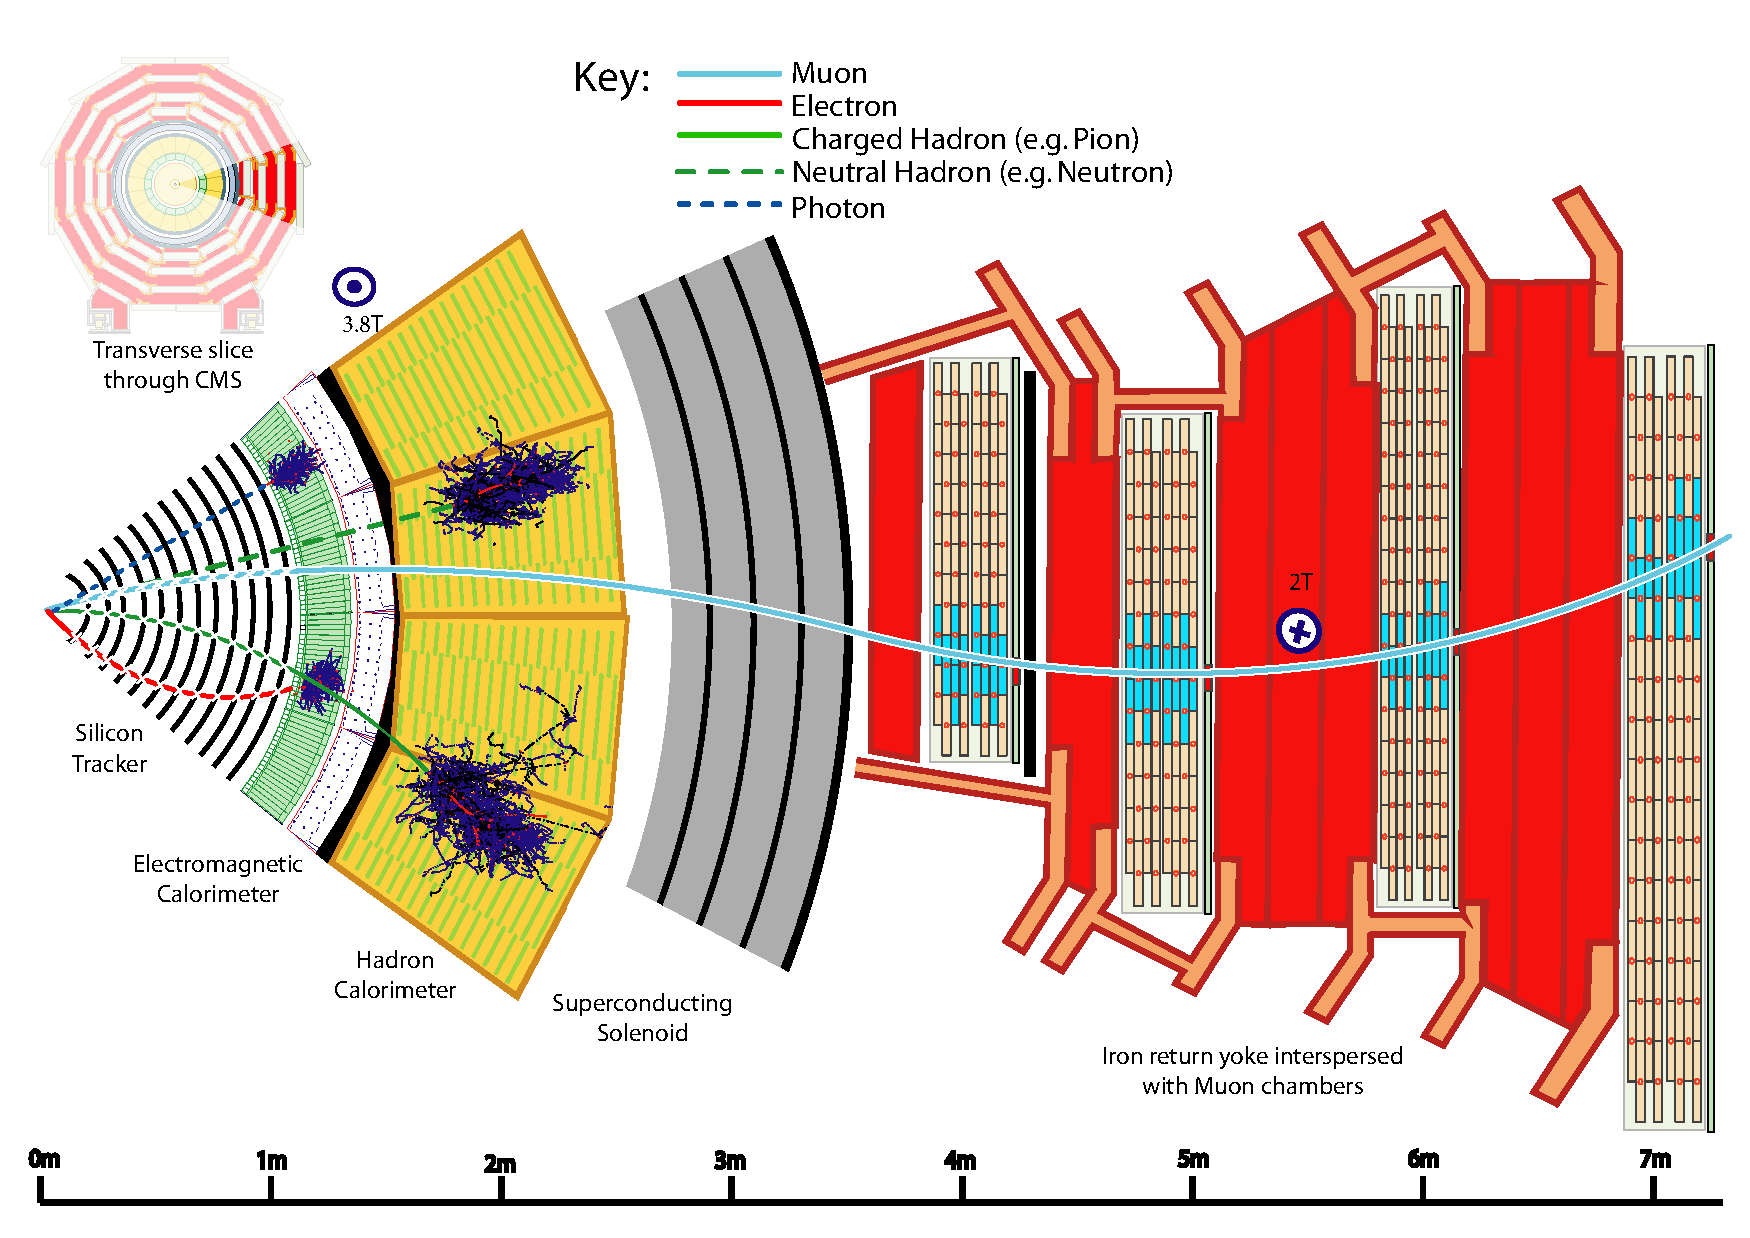
\includegraphics[width=0.6\textwidth]{chapter4/CMS_detecter_slice.pdf}
\caption{A sketch view of CMS detecter. Examples are given to show how the particles interact with different sub-detecters.}
\label{fig:CMSslice}
\end{figure}



\subsection{Muon reconstruction and selection criteria}

PF muon is used in the $\Hmuhad$ analysis. In CMS, the event reconstruction starts from building the tracks in tracker(tracker track) and muon system(standalone-muon track) separately. Global muon reconstruction and tracker muon reconstruction are based on these tracks. ~\cite{muonreco}. Global muon reconstruction starts from the standalone-muon tracks and requires at least two muon station in the muon system. For each of the standalone-muon track, a propagating is done to find a matching tracker track on the common surface. Kalman-filter technique~\cite{Fruhwirth:1987fm} is used in the fitting to combine the hits in standalone-muon track and tracker track. The tracker muon starts from the tracks with $\pt>0.5$GeV and total momentum $p>2.5$ GeV. The tracks are then extrapolated to match the tracks in the muon system with at least one muon segment.  Within the geometry acceptance of muon system, the muon reconstruction efficiency is high, especially high momentum muons, constructed as either global muon or tracker muon or both has the  efficiency about 99\%.  PF reconstruction utilizes the whole detector information to identify and reconstruct all of the particle. The muon PF algorithm applies a series of selections to the global muon and tracker muon to select out the PF muon. The selection is optimized to identify the muons in the jets with high efficiency and low misidentify rate. The details of the selection is in~\cite{PFmuonselection}.   



With the PF muon as the input, muons used in the analysis are further categorized into different identification, isolation categories. Muon ID suggested in CMS RunII, for the LHC data 2016, running period BCDEF, ICHEP medium muon ID is applied(table~\ref{tbl:ICHEPMedID}), for running period G and H, also the monte Carlo samples, standard medium muon ID(table~\ref{tbl:standardMedID})are applied to achieve the best performance for muon identification. 

%In the compatibility-based selection, two ?compatibility? variables are constructed, one based on calorimeter information and the other based on information from the
%muon system. A tracker muon is considered to be a muon candidate if the value of a linear combination of these variables is larger than a pre-defined threshold.
%The segment compatibility, which can have values between 0 and 1, describes the quality of the spatial
%agreement between muon segments and the reconstructed track of the muon candidate


%The kink finder algorithm searches for an interaction of the studied particle with the layers of the
%tracking system by performing a fit of the section of the track before the layer with the one after the
%layer. If an interaction happened, the fit will not work properly because of a change in curvature of
%the track.



\begin{table}[!tpb]
\caption{Muon ID used in the analysis, for the LHC data 2016, running period BCDEF.  \label{tbl:ICHEPMedID}}
\label{tab:antil}
\begin{center}
\begin{tabular}{|l|c|}   
\hline
ICHEP mediumID description                    &  Technical description\\\hline
Loose muon ID                               & PFLoose Muon\\\hline
Fraction of valid tracker hits           & $>0.49$ \\\hline
\multirow{5}{*}{1.Good Global muon}                      &Global muon\\\cline{2-2}
                                                                        &Normalized global-track $\chi^{2}<3$\\\cline{2-2}
                                                                        &Tracker-Standalone position match $< 12$\\\cline{2-2}
                                                                        &kick finder $< 20$ \\\cline{2-2}
                                                                        &Segment compatibility $> 0.303$ \\\hline                                                                       
\hline
2. Tight segment compatibility      & Segment compatibility $>0.451$\\\hline
\end{tabular}
\end{center}
\end{table}


\begin{table}[!tpb]
\caption{Muon ID used in the analysis, for the LHC data 2016, running period G and H, also the monte Carlo samples.  \label{tbl:standardMedID}}
\label{tab:antil}
\begin{center}
\begin{tabular}{|l|c|}   
\hline
Standard mediumID description                    &  Technical description\\\hline
Loose muon ID                               & PFLoose Muon\\\hline
Fraction of valid tracker hits           & $>0.8$ \\\hline
\multirow{5}{*}{1.Good Global muon}                      &Global muon\\\cline{2-2}
                                                                        &Normalized global-track $\chi^{2}<3$\\\cline{2-2}
                                                                        &Tracker-Standalone position match $< 12$\\\cline{2-2}
                                                                        &kick finder $< 20$ \\\cline{2-2}
                                                                        &Segment compatibility $> 0.303$ \\\hline                                                                       
\hline
2. Tight segment compatibility      & Segment compatibility $>0.451$\\\hline
\end{tabular}
\end{center}
\end{table}


\subsection{Electron identification}

Electrons in CMS is constructed with the information from tracker and calorimeters. One of the main difficulties is the bremsstrahlung emitted by the electron during the traveling among the detector materials. The conversion of the photons from the bremsstrahlung affect the reconstruction of tracks in the track and these phones also cause significance energy loose in the electron reconstruction. The construction of Electron is discussed in section~\ref{PFtracker} and more details can be found in~\cite{electron_reco2015}. 

Electron ID is constructed to separate Prompt isolated electron(signal) from the background processes. The background can be the electrons from photon conversion, from quark semi-leptonic decay and from misidentification of other particles or jets. The variables used in the identification are related to tracker and ECAL.  There are mainly three types of variables. The variable related only to calorimeters. For example, the cluster shape of real electron in ECAL is usually narrower than the shape from hardonic showers and electrons leave most of the energy in ECAL and the energy ratio between ECAL and HCAL is large. The variables related to the matching of measured energy and geometry between tracker and ECAL. The variables related to tracker fitting to explore the difference between electrons and hadrons. These related variables can be used to construct cut-based selection sequence to selection electron. To achieve better performance, MVA based ID with boosted decision tree is also trained. Compared with the cut-based selection, more variables in the three categories mentioned above are used in the training~\cite{electron_reco2015}.  An example of the BDT electron ID is shown in Figure.~\ref{fig:eleBDTID}


\begin{figure}[!htbp] 
     \centering
     \subfigure[EB]{ 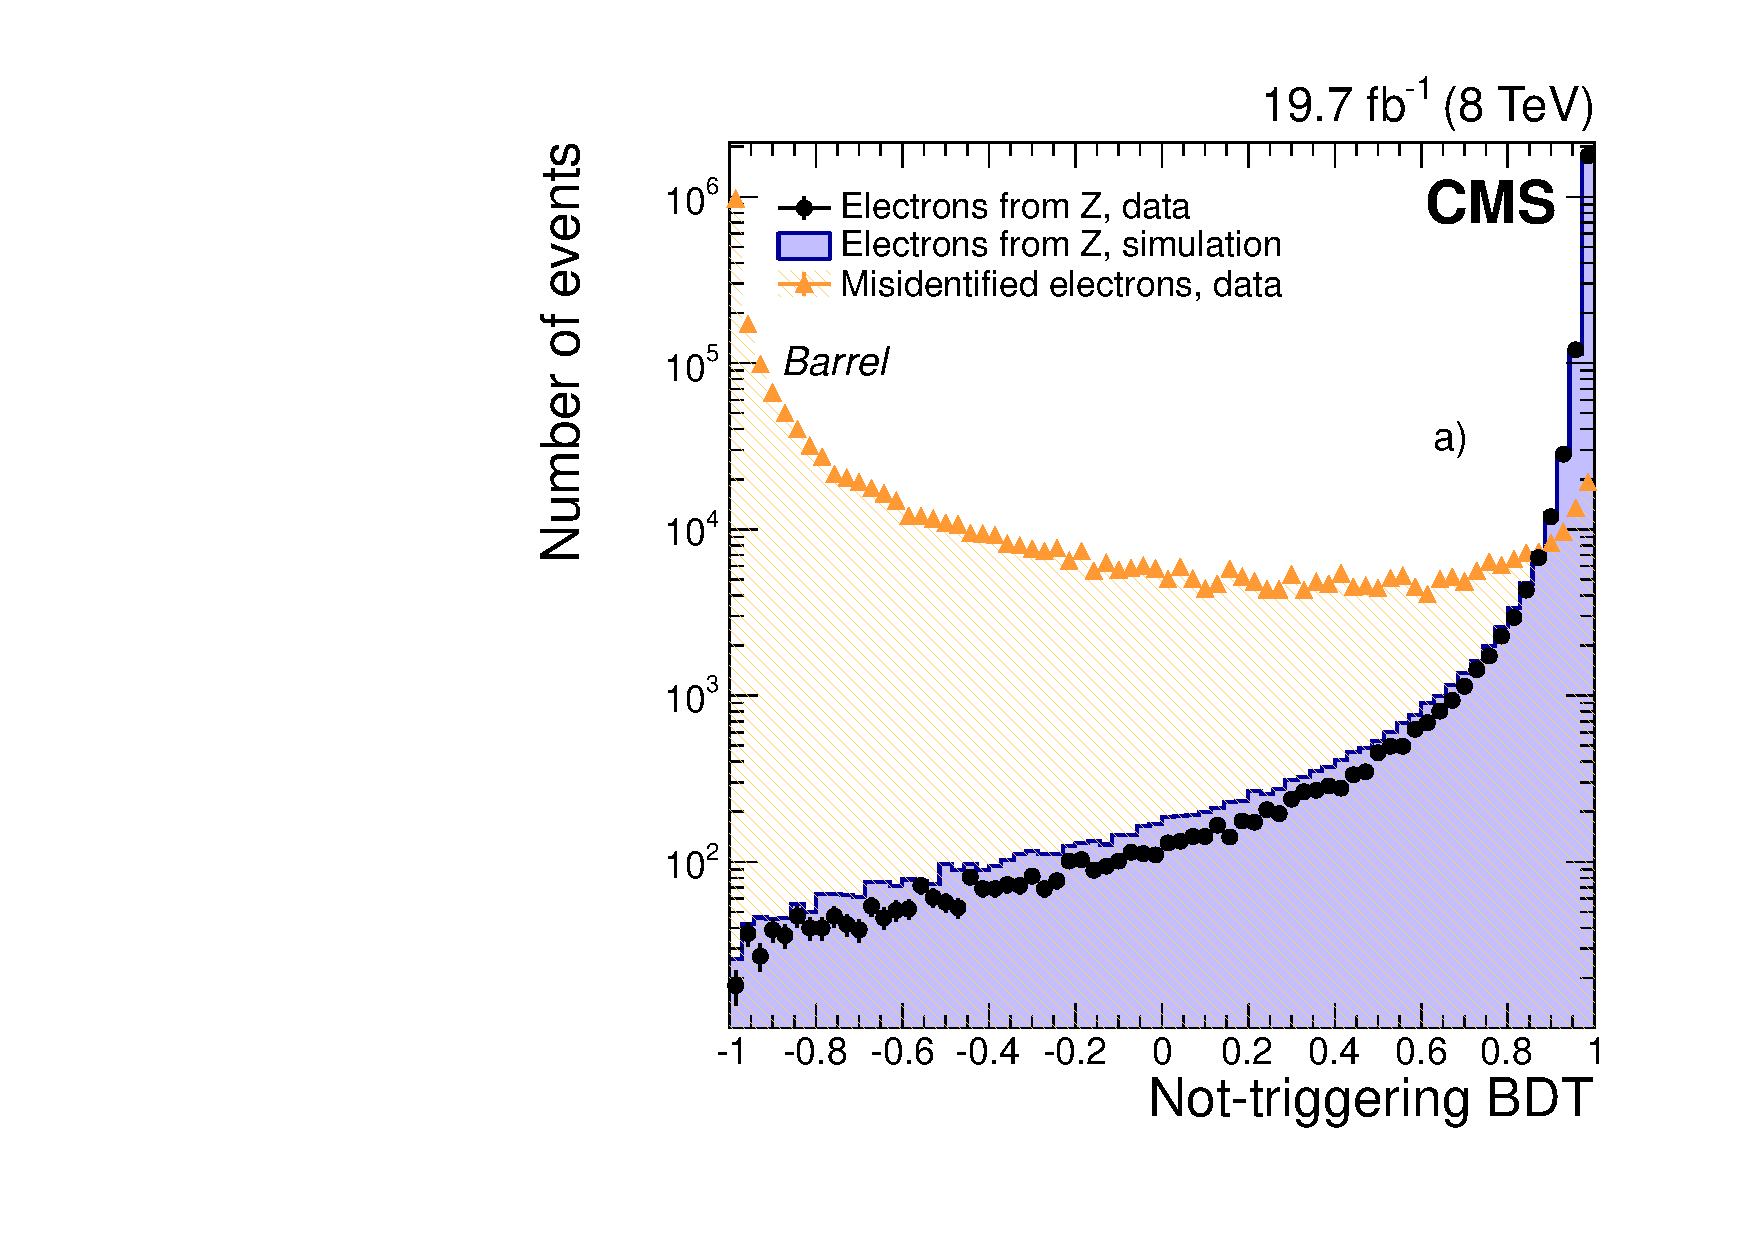
\includegraphics[width=0.4\textwidth]{chapter4/EleID_EB_BDT_perfor.pdf}}
     \subfigure[EE]{ 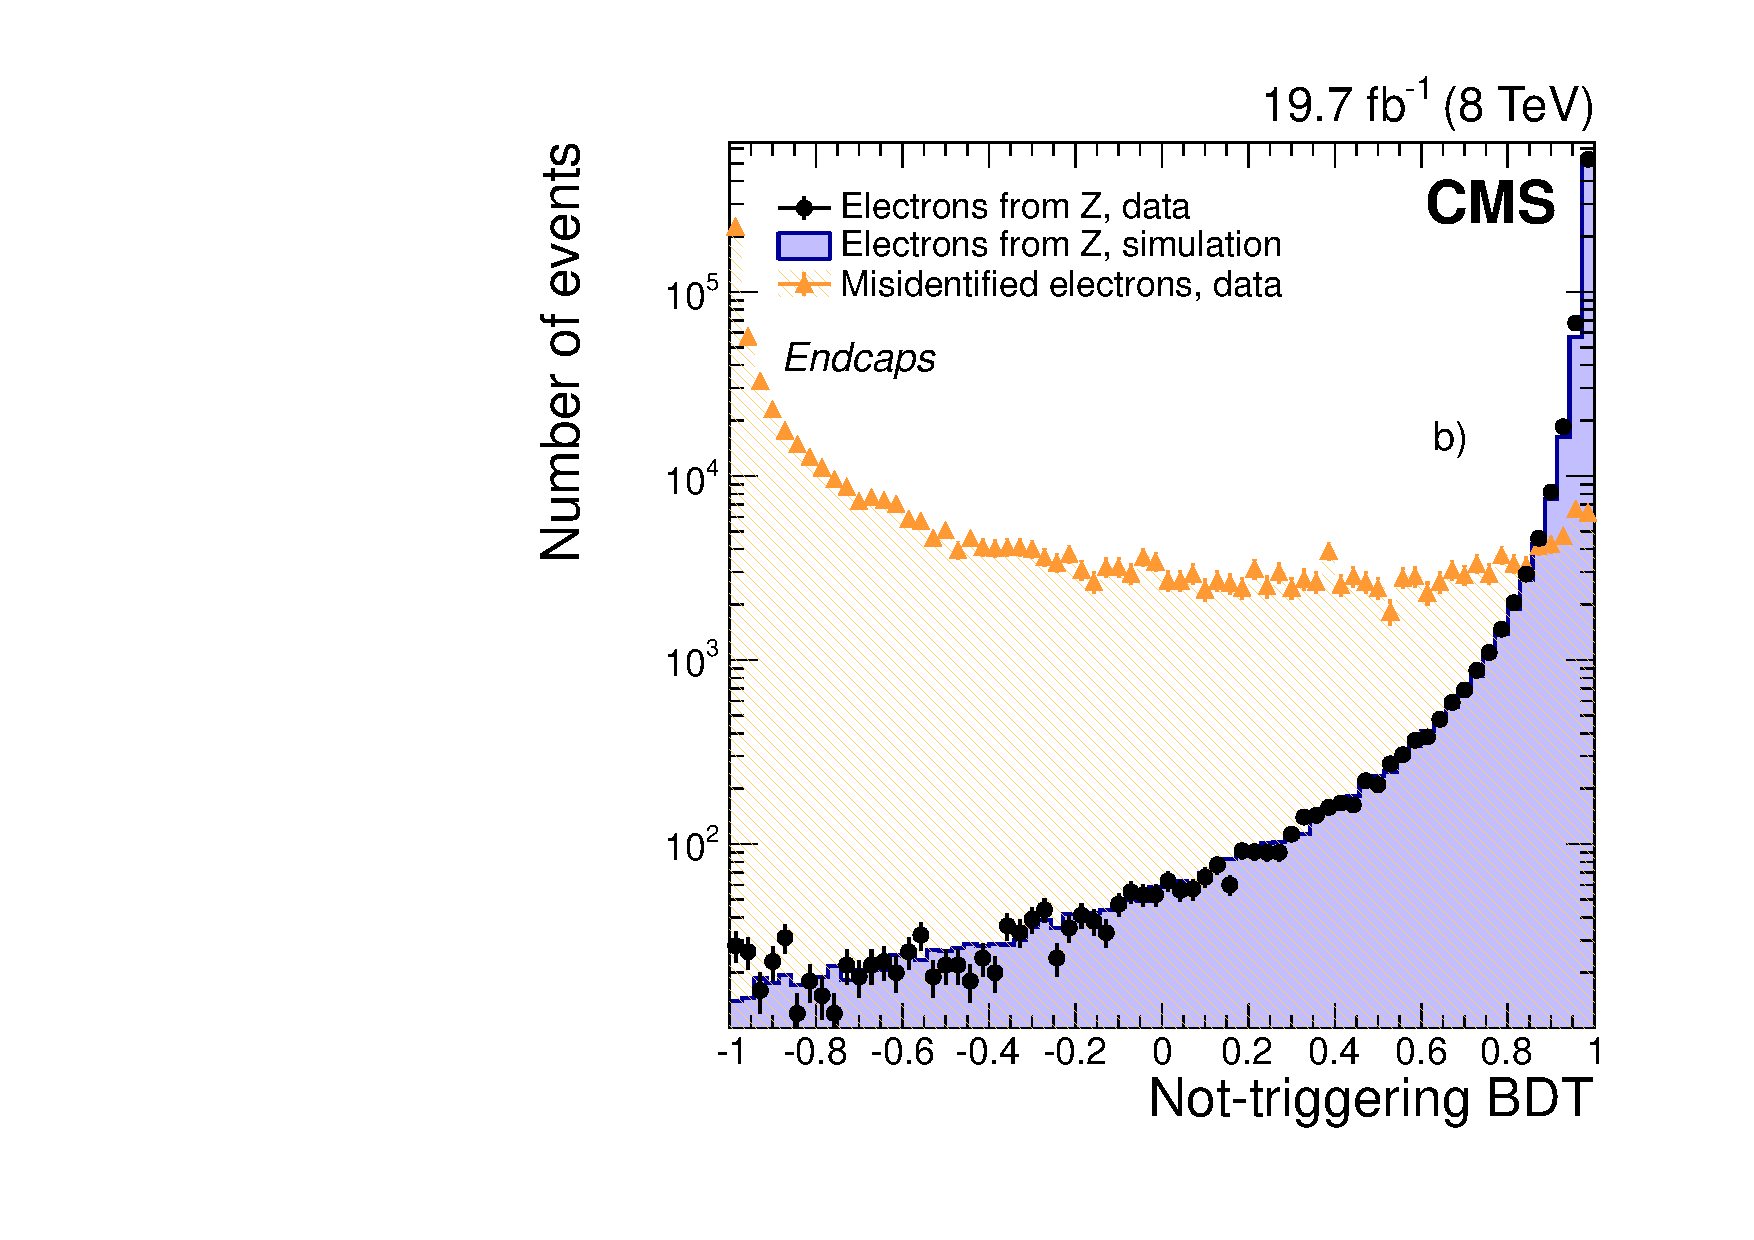
\includegraphics[width=0.4\textwidth]{chapter4/EleID_EE_BDT_perfor.pdf}}\\
     \caption{Electron BDT-based ID shows good discriminating power against background in both EB and EE~\cite{electron_reco2015}}
     \label{fig:eleBDTID}
\end{figure}


Electron isolation is used to reject background events in addition to the ID variables, also inverting the requirement in the isolation can be used to setup enriched background control regions. Large numbers of background events that can possible enter the signal selection are misidentified jets or the jets in which there are real electrons, for example the jets from b quark semi-leptonic decay. For these background events, one key different character with respect to signals is more energy flowing around the electron(or misidentified electron) trajectory. The isolation requirement used in HLT level is summing over the energy depositions either in ECAL or HCAL in the certain core, for example $\Delta R=0.3,0.4$, $\Delta R=\sqrt{\Delta \phi^{2}+\Delta\eta^{2}}$. The contribution from the particle candidate is removed. In the offline algorithm, particles can better identified with the PF algorithm. Similar in concept to the isolation using the energy flow, the PF isolation summing over the $\pt$ of the particles in the direction of the reconstructed candidate trajectory momentum. PF algorithm utilizes the whole detector information and the isolation is defined as

\begin{align*}
\textrm{Iso}_{\textrm{PF}}=\sum \pt^{\textrm{charged}}+\textrm{max}\bigg[ 0,\sum \pt^{\textrm{neutral~had}} +\sum \pt^{\gamma}-\pt^{\textrm{PU}}\bigg]
\end{align*}

The isolation variable sums over the contribution from charged PF candidates, neutral particles and photons in a certain selected $\Delta R$ region around the signal. The contribution from pileup is estimated with $\pt^{\textrm{PU}}$ with the FASTJET technique~\cite{FastJetalso}. The energy of PF objects are better calibrated and the double counting problem which shows up the energy flow isolation described above is solved. PF isolation variable performs better than the isolation variable used in HLT. The performance comparison is shown in Figure.~\ref{fig:eleIso}

\begin{figure}[!htbp] 
     \centering
     \subfigure[EB]{ 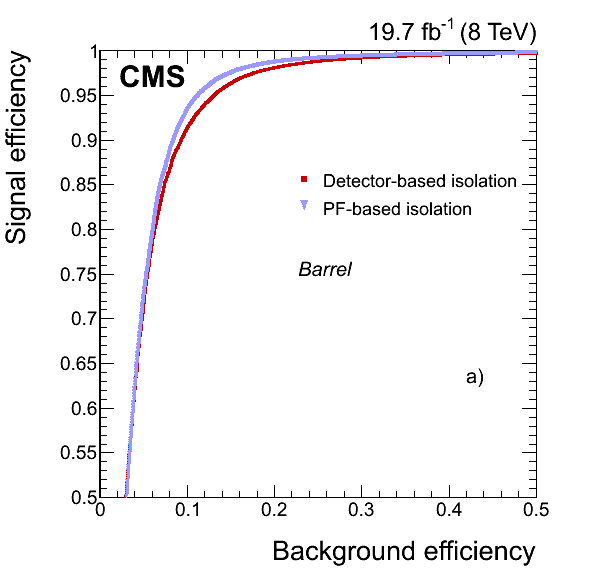
\includegraphics[width=0.4\textwidth]{chapter4/ROC_IsoOnly_Data_EB_HighPt.png}}
     \subfigure[EE]{ 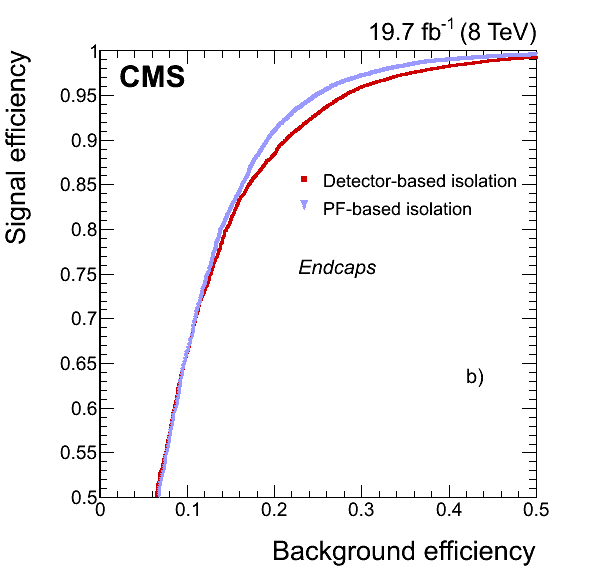
\includegraphics[width=0.4\textwidth]{chapter4/ROC_IsoOnly_Data_EE_HighPt.png}}\\
     \caption{PF electron isolation shows better performance in both EB and EE with respect to detector based isolation variable~\cite{electron_reco2015}}
     \label{fig:eleIso}
\end{figure}


This should be used for B-tagging citation~\cite{BTV-16-002}


\subsection{Tau lepton reconstruction} \label{Chapter:taureco}

In Run I CMS experiment, tau lepton are constructed with hadrons plus strips(HPS) algorithm. In general, HPS starts with PF jets which are reconstructed with $anti-k_{T}$, as the initial seeds. $\pi_{0}$ components from the $\tau$ hadronic decays are first constructed and combined with the charge hadrons parts, to identify different $\tau$ decay modes and calculate $\tau$ four-momentum and other quantities ~\cite{TauIdentiRunI}. 

Photon conversions and the bremsstrahlung of electron/positron when traveling inside the CMS detector are well treated by the HPS algorithm. These phenomenons broaden the signature of the tau decay. With PF jets as input, the algorithm constructs strips out of electromagnetic particles and starts by taking the strip in which contains the most energetic electromagnetic particle as the center one. With the center strip, a window of the size $\Delta \eta=0.05$ and $\Delta \phi=0.2$ is taken. Within this window, if other charged particles are found, they are associated with the strip. The position of the strip is taken and four momentum of the strip is calculated. This procedure is repeated, until no strips can be constructed. The selected strips are required to have $P_{T}^{strip}>1GeV$. The following decay topologies are taking into account by HPS:
\begin{enumerate}[$\bullet$]
\item one charged particle without any strip, $h^{\pm}$ and the case when $\pi^{0}$ is not energetic enough to form a strip
\item one charged particle plus one strip
\item one charged particle plus two strips
\item three charged partibles. 
\end{enumerate} 

All of the charged hadrons and strips are required to be contained in the $\Delta R=2.8/P_{T}^{\tau_{h}}$ core, where the $P_{T}^{\tau_{h}}$ is the reconstructed $\tau_{h}$ transverse momentum and $\Delta R$ is defined as $\Delta R=\sqrt(\Delta \phi^{2}+\Delta \eta^{2})$. The $\tau_{h}$ candidate is also required to match the direction of the seed PF jet within $\Delta R=0.1$. Assuming all of the charged hadrons to be pions and taking in the associated strips, the HPS algorithm requires that different decay topologies meet the intermediate meson mass as listed in Table.~\ref{tb:tauHdecay}. 

The cut based $\tau_{h}$ isolation discriminant required that the PF charged particles and photons to be considered in the isolation variable have $\pt>0.5$ GeV and within an isolation cone  $\Delta R=0.5$ in $\tau_{h}$ direction. The particles that  constituent $\tau_{h}$ are excluded from the summation. The effect of charged particle from pileup is eliminated by considering on the charged particle oriented from the $\tau_{h}$ production vertex with in $D_{z}=0.2$ cm and $\Delta r=0.03$ cm. The effect of pileup on the isolation of the photons on the strips is estimated by summing the charged particles that are not oriented from $\tau_{h}$ decay primary vertex, within $\Delta R=0.8$ cm in the direction of and have the impact parameter $D_{z}>0.2$ cm. Then a factor $\Delta \beta$ is multiplied to the $\pt$ sum. The isolation variable is defined as in Equation.~\ref{eq:taucutiso1}.

\begin{align}
I_{\tau}=\sum \pt^{\text{charged}} (d_{z}<0.2 \ \text{cm})+\text{max}(0,\sum \pt^{\gamma}-\Delta \beta \sum \pt^{\text{charged}} (d_{z}>0.2 \ \text{cm}))\label{eq:taucutiso1}
\end{align}

Tight, loose, medium working points(WP) for the tau isolation discriminants. The exact of the energy selection is suggested by the study of QCD dijet events, by requiring the $I_{\tau}$ in Equation.~{eq:taucutiso1} to have different values. The loose cut brings in approximate $1\%$ of fake $\tau$ from jets. 


\begin{table}[htp]
\caption{Dominant hadronic $\tau$ lepton decays branching fractions and the associated intermediate resonance. The h stands for both $\pi$ and K. The table is symmetric under charge conjugation.}\label{tb:tauHdecay}
\begin{center}
\begin{tabular}{|c|c|c|c|}
\hline
Decay mode                                             & Resonance & Mass ($MeV/c^{2}$) & Branching fraction(\%)\\\hline
$\tau^{-}\to h^{-}v_{\tau}$                                     &                                  &           &  11.6\%     \\
$\tau^{-}\to h^{-}\pi^{0} v_{\tau}$                       & $\rho^{-}$                 & 770     &   26.0\%      \\
$\tau^{-}\to h^{-}\pi^{0} \pi^{0}  v_{\tau}$       & $\alpha_{1}^{-}$       & 1200   &   9.5\%     \\
$\tau^{-}\to h^{-}h^{+}h^{-}v_{\tau}$                     & $\alpha_{1}^{-}$       &  1200  &   9.8\%  \\
$\tau^{-}\to h^{-}h^{+}h^{-}\pi^{0} v_{\tau}$      &                                  &            &   4.8\% \\\hline
 \end{tabular}
\end{center}
\end{table}


In CMS Run II, Tau reconstruction algorithm HPS has been improved~\cite{TauRecoandIDRunII}. The major improvement lies in Dynamic strip instead of fix size strip. Tau decay products can also affect the isolation. Charged pions in tau decay products experience nuclear interaction with tracker materials, which can results in low $P_{T}$ secondary particles. Photons from the neutral pion decay can also go through pair production into $e^{+}e{-}$, which further spread because of bremsstrahlung and the magnetic field. Broadening the strip is need in these cases in order to better cover the tau decay production. On the other hand, if the tau is boosted, high $P_{T}$ decay products tends to be more concentrate and smaller strip size will be better. Similar to RunI tau reconstruction, the algorithm starts with hightest $\pt$ charged particle as seeds for the strip. Starting from the seed strip, a window in $\eta$ and $\phi$ direction is set.  

\begin{align*}
\delta\eta&=f(P_{T}^{\gamma})+f(P_{T}^{strip})   & f(P_{T})&=0.2\cdot P_{T}^{-0.66}\\
\delta\phi&=g(P_{T}^{\gamma})+g(P_{T}^{strip}) & g(P_{T})&=0.35\cdot P_{T}^{-0.71}\\
\end{align*}

The window is determined from single $\tau$ gun MC simulation. 95\% of the decay product will be covered in that range. The upward and downward limits for $\eta$ is 0.15 and 0.05, for $\phi$ the range is 0.3 and 0.05.  The position of strip is set as $\pt$ weighted average against all of the objects. 

\begin{align*}
\eta_{strip}&=\frac{1}{P_{T}^{strip}}\cdot\sum P_{T}^{\gamma}\cdot\eta_{\gamma}\\
\phi_{strip}&=\frac{1}{P_{T}^{strip}}\cdot\sum P_{T}^{\gamma}\cdot\phi_{\gamma}\\
\end{align*}

Construct the strip until no seed strip can be found. After the construction of the $\tau$ lepton, for different decay mode, $m_{\tau}$ is required to lie in different mass windows~\cite{TauReconstuction}.  The conditions of different hadronic decay mode mass window are listed in the Table.~\ref{tb:tauHdecayRecomass}. With respect to RunI, the difference in mass window is $\delta m$, which originates from dynamic clustering. $\delta m$ is calculated as:

\begin{align*}
\delta m&=\sqrt{\Big(\frac{\partial m_{\tau}}{\partial \eta_\text{{strip}}}\cdot f(\pt^\text{{strip}})\Big)^{2}+\Big(\frac{\partial m_{\tau}}{\partial \phi_\text{{strip}}}\cdot g(\pt^\text{{strip}})\Big)^{2}}\\
\end{align*}
with:
\begin{align*}
\frac{\partial m_{\tau}}{\partial\eta_{strip}}&=\frac{P_{z}^{strip}\cdot E_{\tau}-E_{strip}\cdot P_{z}^{\tau}}{m_{\tau}}\\
\frac{\partial m_{\tau}}{\partial\phi_\text{{strip}}}&=\frac{-(P_{y}^{\tau}-P_{y}^\text{{strip}})\cdot P_{x}^\text{{strip}}+(P_{x}^{\tau}-P_{x}^\text{{strip}})\cdot P_{y}^\text{{strip}}}{m_{\tau}}
\end{align*}


\begin{table}[htp]
\caption{$\tau$ hadronic decay mode hypothesis signatures compatibility tests. $m_{\tau}$ is required to be in the mass window }\label{tb:tauHdecayRecomass}
\begin{center}
\begin{tabular}{|c|c|}
\hline
Decay mode                                             & Mass window\\\hline
$\tau^{-}\to h^{-}\pi^{0} v_{\tau}$                       & $0.3-\delta m_{\tau}<m_{\tau}<1.3\cdot \sqrt{\pt/100}+\delta m_{\tau}$      \\\hline
$\tau^{-}\to h^{-}\pi^{0} \pi^{0}  v_{\tau}$       &  $0.4-\delta m_{\tau}<m_{\tau}<1.2\cdot \sqrt{\pt/100}+\delta m_{\tau}$   \\\hline
$\tau^{-}\to h^{-}h^{+}h^{-}v_{\tau}$                     & $0.8-\delta m_{\tau}<m_{\tau}<1.5+\delta m_{\tau}$   \\\hline
 \end{tabular}
\end{center}
\end{table}

In current algorithm, $\tau^{-}\to h^{-}h^{+}h^{-}v_{\tau}$ is not included, because of the jets contamination. This hadronic $\tau$ decay mode composed of 4.8\% of total branching fraction. The $h^{-}\pi^{0}$ and $h^{-}\pi^{0}\pi^{0}$ are analyzed together, which is referred as $h^{-}\pi^{0}$.

The analysis with 2016 datasets, MVA based $\tau$ isolation criteria is used, which keeps high identification efficiency while maintains relatively low fake rate compared with cut based discriminator. A Boosted Decision Tree(BDT) has been used in the training of the isolation variable. With BDT, the isolation variable shows a good distinguishing power against jets. Various variables have been used as BDT inputs. The variables are isolation variable($I_{\tau}$), impact parameter from highest $\pt$ track of $\tau_{h}$ candidate, $\tau_{h}$ decay mode information, shape variables like $\Delta R$, $\Delta \eta$, $\tau-$lifetime information and photon electron multiplicity, more of the exact variables used are discussed in~\cite{TauRecoandIDRunII,TauReconstuction}. BDT uses these variables to distinguishing $\tau_{h}$ dacay($H \to \tau \tau$) from jets, which can be the decay products from quarks and gluons(QCD MC).  

BDT method also used in the tau discriminating again electron training. The algorithm utilizes the variables that sensitive to the energy deposit in Ecal and Hcal, the electron bremsstrahlung, overall particle multiplicity and difference in electromagnetic and hadronic showers. Detail list of variable can be find in~\cite{TauRecoandIDRunII,TauReconstuction}.

Tau signals can be faked by muons, especially in $\tau_{h}$ decay mode $h^{\pm}$. Tau against muon cut based muon discriminant is set by checking if there are signals in the muon system within $\Delta R=0.3$ of the $\tau_{h}$ direction or if the energy sum from Ecal and Hcal is less than 20$\%$ of the total $\tau$ energy. If less than two hits are found in the muon system, then it passes the loose working point. If no hits are found in the muon system, then this is the tight working point. 

\subsection{Jet reconstruction}


Anti-$k_{t}$ jet clustering algorithm~\cite{Cacciari:2008gp} is used in CMS for the jet reconstruction. The algorithm starts by introducing the distance $d_{ij}$ and $d_{iB}$ as following,

\begin{align*}
d_{ij}&=min(k_{ti}^{2p},k_{tj}^{2p})\frac{\Delta_{ij}^{2}}{R^{2}}\\
d_{iB}&=k_{ti}^{2p}
\end{align*}

$d_{ij}$ is the distance between entities, the particle and the pseudojet. $\Delta_{ij}$ is the difference of rapidity and azimuth between entry i and entry j. $\Delta_{ij}^{2}=(\eta_{i}-\eta_{j})^{2}+(\phi_{i}-\phi_{j})^{2}$. R is a radius parameter. $k_{ti}$ and $k_{tj}$ stands for the momentum of the entries respectively. p is a parameter used to specify jet construction algorithms.  For Anti-$k_{t}$, p=-1. $d_{iB}$ is the distance between entry i and the beam. If the parameter p is set for other values, for example p=1 or 0, then the algorithm is the $k_t$~\cite{ktalgo} or Cambridge/Aachen jet reconstruction algorithm~\cite{Aachenjetalgo}.  With the Anti-$k_{t}$, assuming in one event, there are a couple hard particle with high momentum, $k_{t1}$, $k_{t2}$ and so on, also large numbers of soft ones around. Starting from $k_{t1}$ as an example, if $d_{1j}$ is smaller, then entry j combined with entry 1, if $d_{1B}$ is smaller, then entry 1 is set as a jet and removed from the list. The soft entries tend to ground around the high momentum entries to the range $\Delta_{ij}= R$, if there is no other hard entry around. If two hard entries are within the distance R, then the two entries are clustered into a single entry. In this case, if $k_{1}\gg k_{2}$, then the center is more closed to jet 1. If $k_{1}\sim k_{2}$, the boundary between to two jets is defined by $\Delta R_{1b}/k_{t1}=\Delta_{2b}/k_{t2}$. Jet clustering continues until all of the jets are clustered in the events. 

Jet energy is corrected to have the correct energy scale.  The correction goes through a couple of steps~\cite{jetenergycorrection}. The major corrections are derived from simulated samples and the residual corrections from the different response between MC and data are from data-driven methods. 

Pileup events can increase the measured jet energy, especially in LHC Run II, the number of pileup per event doubled. Two types of pileup affect the performance the most, in-time pileup(IT PU) and out-of time pileup(OOT PU). The IT PU refers to the additional events produced by the proton-proton collision within the same bunch-crossing as the primary hard collision.   The OOT PU refers to the events that produced in previous bunch crossing or subsequent one that affect current bunch. OOT PU can be mitigated by explore the timing window, pulse shape of the calorimeter. The IT PU mitigation is mainly discussed. Charged hadrons from IT PU in CMS are removed with Charged-hadron subtraction(CHS) algorithm in CMS. Tracks with the vertexes that are identified from PU with charged particles inside are removed. CHS removes around 50\% of the IT PU within the tracker coverage region. There are also soft jets from pileup interaction. These jets are usually in low energy range and affects the JES by overlapping with the hard jets. Multivariate analysis(MVA) with inputs from jet shape and jet constitution information can more than 90\% of pileup jets. This MVA ID is referred as PUJetID~\cite{PU_jetID}. After rejecting the charged particle jets and soft jets from pileup, a jet area method~\cite{FastJetalso} is used to further eliminate the effects from PU. In this method, an estimated energy density bringing in by the PU and effective area of jet is used to calculate the offset energy. After the PU correction, a matching between particle-level jets and reconstructed jets is performed with MC samples for the simulated response corrections. 









\section{Event simulation}

